\subsubsection{Paketdiagramm}

Die LasEs-Anwendung verwendet eine Vierschichtenarchitektur.
\begin{itemize}
    \item Die \emph{view}-Schicht enthält die Komponenten zur grafischen Darstellung.
    \item Die \emph{control}-Schicht enthält die Komponenten zur Steuerung der grafischen Darstellung und Reaktion auf
    Nutzereingaben.
    \item Die \emph{business}-Schicht enthält die Komponenten, welche die Anwendungslogik umsetzen.
    \item Die \emph{persistence}-Schicht enthält die Komponenten zum Zugriff auf den Datenbankserver.
\end{itemize}
Diese Schichten folgen der \emph{\hyperref[arch:mvc]{MVC-Architektur}} wie in
\textbf{\hyperref[feinarch:pakdia]{Abbildung 1}} dargestellt.
Die \hyperref[arch:persistence]{Persistenz-} und
\hyperref[arch:business]{Businessschichten} gehören hierbei
dem \emph{Model} an. Die \hyperref[arch:control]{Kontrollschicht} stellt den \emph{Controller} und die
Faceletschicht die \emph{View} dar.
\begin{figure}[H]
    \centering
    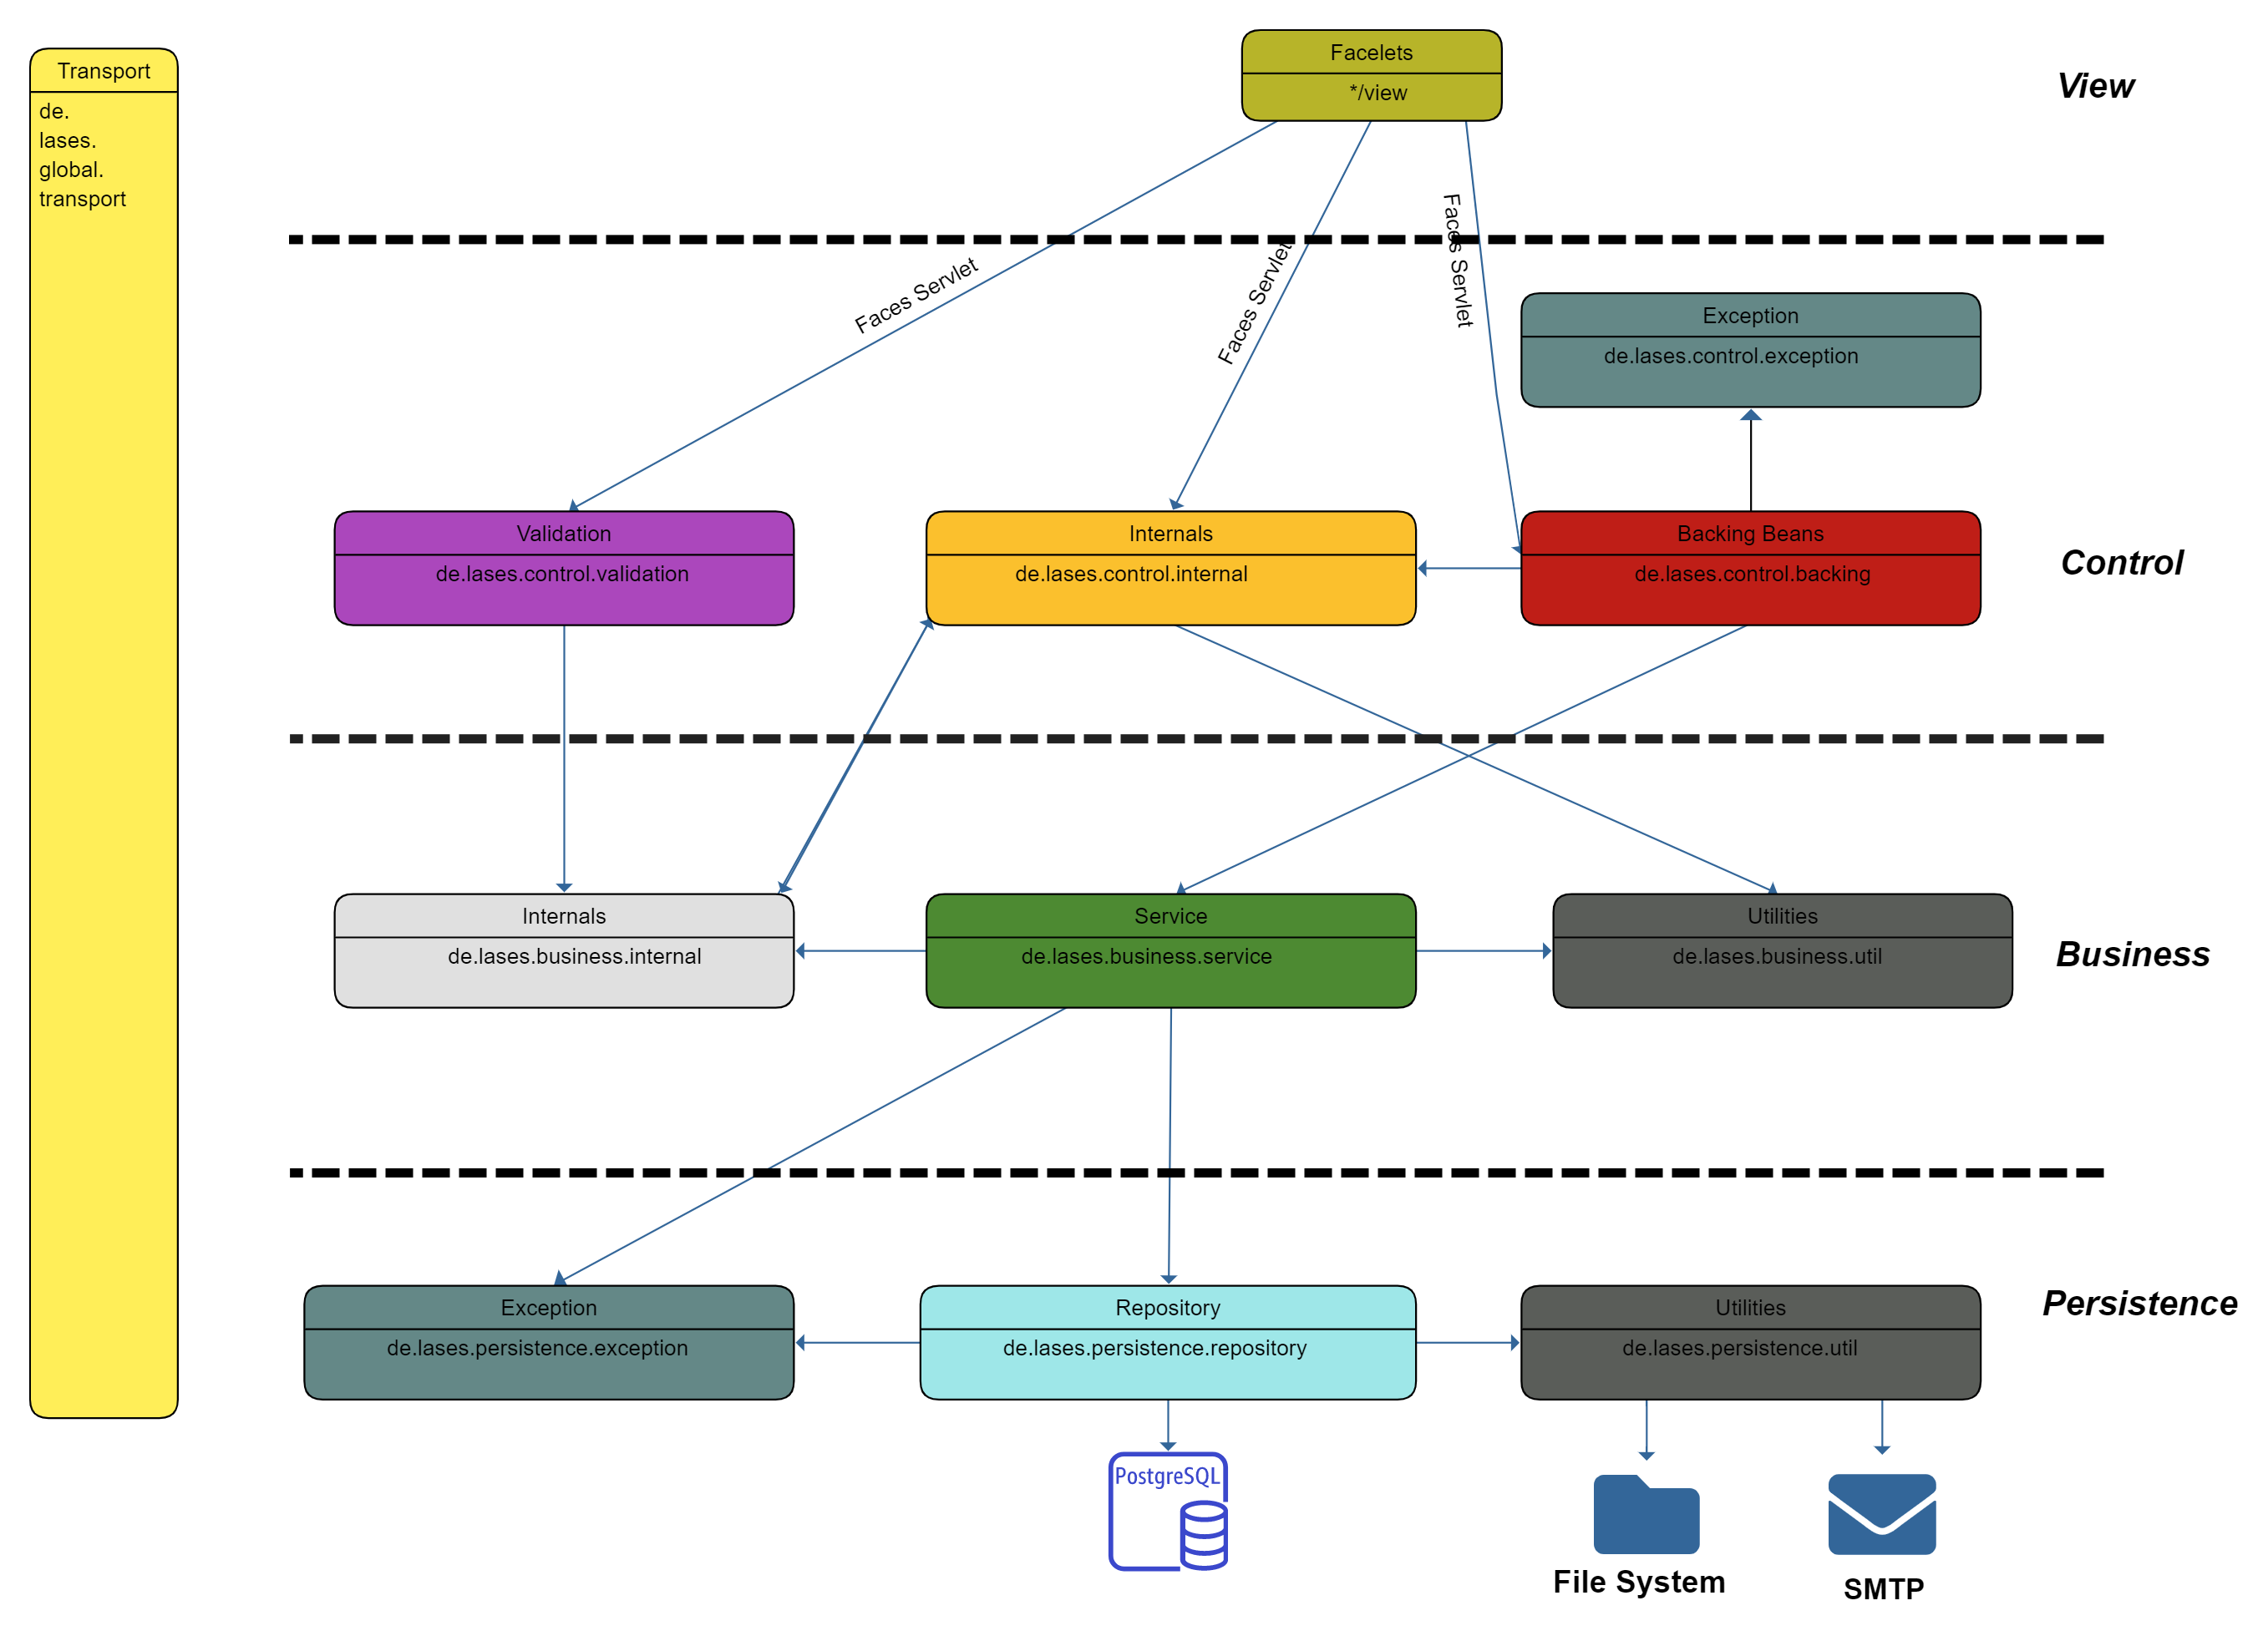
\includegraphics[width=0.8\linewidth]{graphics/Paketdiagramm11.0}\label{feinarch:pakdia}
    \caption{Die Pakete der LasEs-Anwendung.}
\end{figure}

Eine Schicht kommuniziert jeweils nur mit direkt angrenzenden Schichten.
Diese Kommunikation (also der Datenfluss) erfolgt mittels \emph{Data Transfer Objects}.
Somit sind diese eine Ausnahme von der Schichtenarchitektur, da Sie sich keiner
einzelnen Schicht zuordnen lassen.
\emph{DTO}s sind ein schichtenübergreifender \emph{cross-cutting concern}.

\subsubsection{Ordnerstruktur}

Die Ordnerstruktur dieser Anwendung ist ausgelegt auf klare Trennungen und Übersichtlichkeit.
In \hyperref[feinarch:orddia]{Abbildung 1} werden Quellcodedateien ausgespart.

\begin{figure}[H]
    \centering
    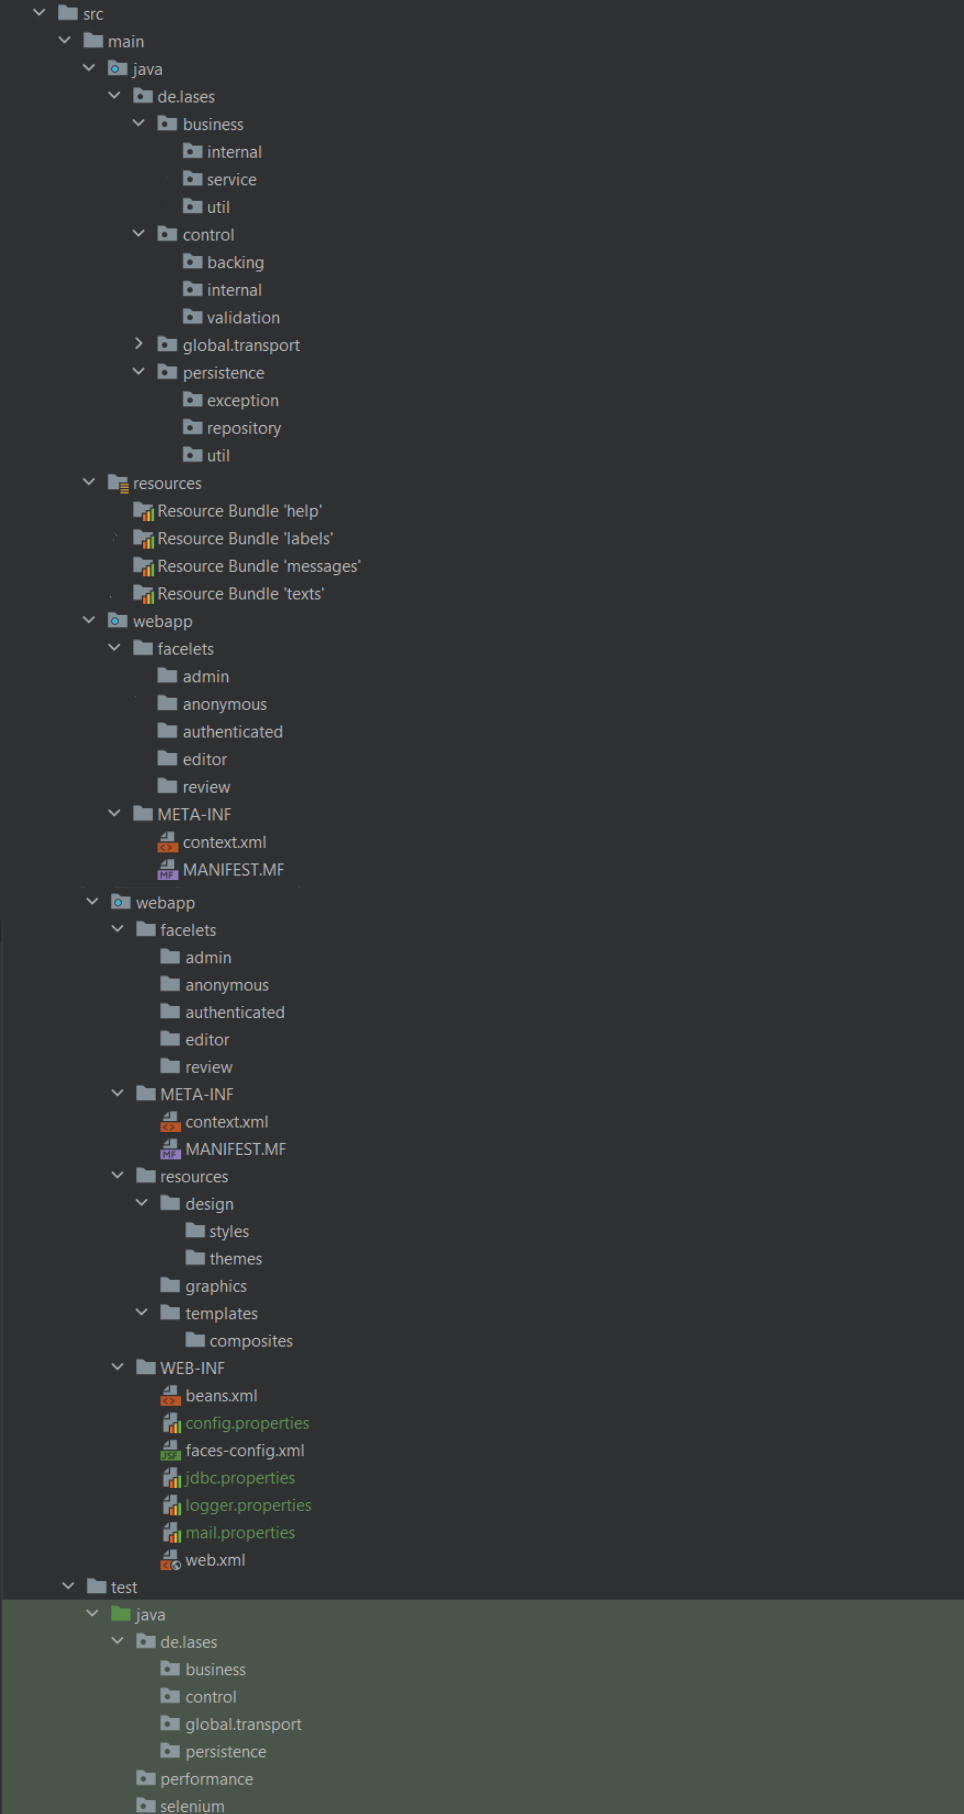
\includegraphics[width=0.8\linewidth]{graphics/folder_structure}\label{feinarch:orddia}
    \caption{Die Ordner- und Dateistrukur der LasEs-Anwendung.}
\end{figure}

\todo{Weißer Hintergrund}